\documentclass[10pt]{beamer}
\usetheme{Goettingen}
%\usetheme{AnnArbor}
%\setbeamercolor{palette sidebar secondary}{fg=yellow,bg=blue}
%\setbeamercolor{section in sidebar shaded}{fg=red,bg=black}
%\useoutertheme[right]{sidebar}
%\setbeamersize{sidebar right width=2.5cm}
\setbeamersize{
	text margin left    = .04\paperwidth,
	text margin right   = .04\paperwidth,
	sidebar width left  = 0mm,
	sidebar width right = 20mm,
	description width   = 10mm,
	mini frame size     = 1mm,
	mini frame offset   = 0mm
}
\addtobeamertemplate{navigation symbols}{}{%
	\usebeamerfont{footline}%
	\usebeamercolor[fg]{footline}%
	\hspace{1em}%
	\insertframenumber/\inserttotalframenumber
}

\makeatletter
\setbeamertemplate{sidebar \beamer@sidebarside}
{
	\beamer@tempdim=\beamer@sidebarwidth%
	\advance\beamer@tempdim by -6pt%
	\vskip4em%
	\insertverticalnavigation{\beamer@sidebarwidth}%
	\vfill
	\ifx\beamer@sidebarside\beamer@lefttext%
	\else%
	\usebeamercolor{normal text}%
	\llap{\usebeamertemplate***{navigation symbols}\hskip0.1cm}%
	\vskip2pt%
	\fi%
}%

\ifx\beamer@sidebarside\beamer@lefttext%
\defbeamertemplate*{sidebar right}{sidebar theme}
{%
	\vfill%
	\llap{\usebeamertemplate***{navigation symbols}\hskip0.1cm}%
	\vskip2pt}
\fi

\setbeamertemplate{section in sidebar}%{sidebar theme}
{%
	\vbox{%
		\vskip1ex%
		\beamer@sidebarformat{3pt}{section in sidebar}{\insertsectionheadnumber
			~\insertsectionhead}%
	}%
}
\setbeamertemplate{section in sidebar shaded}%{sidebar theme}
{%
	\vbox{%
		\vskip1ex%
		\beamer@sidebarformat{3pt}{section in sidebar shaded}{\insertsectionheadnumber
			~\insertsectionhead}%
	}%
}
\makeatother
\usepackage{standalone} 

\usepackage{enumerate}
\usepackage{amsmath}%
\usepackage{amsfonts}%
\usepackage{amssymb}
\usepackage{amsthm}%
\usepackage{graphicx}
\usepackage{mathtools}

\usepackage[utf8]{inputenc}
\usepackage[T1]{fontenc}

\usepackage[french]{babel}
\usepackage{caption}
\usepackage{enumerate}
\usepackage{multirow}
\usepackage{aliascnt}
\usepackage{etoolbox}

\usepackage{hyperref}
\addto\extrasfrench{%
	\def\chapterautorefname{chapitre}%
	\def\sectionautorefname{section}%
	\def\subsectionautorefname{sous-section}%
	\def\subsubsectionautorefname{Paragraphe}%
	\def\paragraphautorefname{Paragraph}%
	\def\subparagraphautorefname{Subparagraph}%
	\def\alignautorefname{}
}



\newcommand{\id}{\mathrm{Id}}
%\usepackage[pdftex]{tulhypref}
%\usepackage[pdftex,colorlinks=true,linkcolor=red,bookmarks=false]{tulhypref}
% Ensembles R, C, N, Z et D
\newcommand{\R}{\mathbb{R}}
\newcommand{\C}{\mathbb{C}}
\newcommand{\N}{\mathbb{N}}
\newcommand{\Q}{\mathbb{Q}}
\newcommand{\D}{\mathbb{D}}
\newcommand{\Z}{\mathbb{Z}}
\newcommand{\K}{\mathbb{K}}
\newcommand{\s}{\mathbb{S}}
\newcommand{\A}{\mathbb{A}}
\newcommand{\T}{\mathbb{T}}
\newcommand{\OO}{\mathcal{O}}
\newcommand{\PP}{\mathcal{P}}
\newcommand{\MM}{\mathcal{M}}
\newcommand{\LL}{\mathcal{L}}
\newcommand{\NN}{\mathcal{N}}
\newcommand{\DD}{\mathcal{D}}
\newcommand{\BB}{\mathcal{B}}
\newcommand{\RR}{\mathcal{R}}
\newcommand{\CC}{\mathcal{C}}
\newcommand{\FF}{\mathcal{F}}
\newcommand{\GG}{\mathcal{G}}
\newcommand{\TT}{\mathcal{T}}
\newcommand{\UU}{\mathcal{U}}
\newcommand{\VV}{\mathcal{V}}
%\renewcommand{\thepart}{\Arabic{part}}
\newcommand{\ps}[1]{\left< #1 \right>}
\newcounter{dader}[section]
\renewcommand{\thedader}{\thesection.\arabic{dader}}
\theoremstyle{plain}
\newaliascnt{thms}{dader}
\newtheorem{thm}[thms]{Theorem}
\aliascntresetthe{thms}%[section]
\newtheorem*{thm*}{Theo}
%\theoremstyle{theorem}

% numérotés par section
\newaliascnt{prop}{dader}
\newtheorem{prop}[prop]{Proposition}
\aliascntresetthe{prop}%[section]
\newtheorem{lemme}[dader]{Lemme}%[section]
\newtheorem*{lemme*}{Lemme}
\newaliascnt{cor}{dader}
\newtheorem{cor}[cor]{Corollaire}
\aliascntresetthe{cor}
%[section]
\newtheorem*{corollaire}{Corollaire}
\theoremstyle{definition}
\newtheorem{de}{Definition}
%\aliascntresetthe{de}%[section]
\BeforeBeginEnvironment{de}{%
	\setbeamercolor{block title}{fg=black,bg=blue!25!white}
	\setbeamercolor{block body}{fg=blue, bg=blue!5!white}
}
\AfterEndEnvironment{de}{
	\setbeamercolor{block title}{use=structure,fg=structure.fg,bg=structure.fg!20!bg}
	\setbeamercolor{block body}{parent=normal text,use=block title,bg=block title.bg!50!bg, fg=black}
}
\newtheorem*{defff}{Définition}
%[section]
\newtheorem*{conv}{Convention}
\newtheorem*{nota}{Notation}

\newaliascnt{app}{dader}
\newtheorem{application}[app]{Application}
\aliascntresetthe{app}%[section]
\newtheorem*{terminologie}{Terminologie}
%\theoremstyle{remark}
\newtheorem{rem}[dader]{Remark}
\newaliascnt{ex}{dader}

%[section]
\newtheorem{ex}[ex]{Exemple}
\aliascntresetthe{ex}%[section]
\newtheorem{ctrex}[dader]{Contre-exemple}%[section]

%\usepackage[all]{xy}
\usepackage{pgf,tikz}
\usetikzlibrary{decorations.markings,arrows,backgrounds,automata,calc,patterns,shapes.arrows}
\usetikzlibrary{decorations.markings,arrows,backgrounds,automata,calc,shapes.arrows}

%\let\endtitlepage\relax 
\author{Pierre-Henry COLLIN\\Camille Jardel}
\title{Présentation de l'article:\\ \emph{Directional Modelling of Extreme Wind Speed}}
\titlegraphic{
\includegraphics[scale=.25]{logoiecl.jpg}
\includegraphics[scale=0.3]{UL_LOGO.jpg}}
%\setbeamercovered{transparent} 
%\setbeamertemplate{navigation symbols}{} 
%\logo{} 
\institute{IECL} 
\date{Metz, le 25 Janvier 2022} 
\AtBeginSection[]{
	\begin{frame}{}
		\small \tableofcontents[currentsection, hideothersubsections]
	\end{frame} 
}

\setbeamercolor{block title}{bg=red!30,fg=black}
\setbeamertemplate{blocks}[rounded][shadow=true]
\newtheorem{examplefirst}{Example}
\newtheorem{examplesecond}{Example}
\newenvironment<>{examplefirst}[1][]{%
	\setbeamercolor{block title example}{fg=white,bg=blue!25!white}%
	\begin{example}#2[#1]}{\end{example}}
\newenvironment<>{examplesecond}[1][]{%
	\setbeamercolor{block title example}{fg=white,bg=blue!75!black}%
	\begin{example}#2[#1]}{\end{example}}






\usepackage{pgf,tikz}
\usetikzlibrary{decorations.markings,arrows,shapes.arrows,backgrounds,automata,positioning,calc,patterns,decorations.pathreplacing}
\tikzset{
	side by side/.style 2 args={
		line width=2pt,
		#1,
		postaction={
			clip,postaction={draw,#2}
		}
	}
}
			
			
			\newcommand{\vabs}[1]{\left\vert #1 \right\vert}
			%\newcommand{\norme}[1]{\left\Vert #1 \right\Vert}
			
			
			
			
			
			
			
		%	\addbibresource{bibli1.bib}
			\begin{document}
				
				
				
				
				
				\begin{frame}
					\titlepage
				\end{frame}
				\begin{frame}{Sommaire}
					\tableofcontents
				\end{frame}
				
				\section{Introduction}
				
				%\subsection{Premières définitions}
				
			\begin{frame}{\thesection{} -  \secname}
			\begin{itemize}[<+->]
				\item La vitesse extrême des vents a déjà été modélisée;
				\item Les données de vitesses moyenne et maximale sont connues, ainsi que la composante directionnelle principale.
			\end{itemize}
			\end{frame}
			\begin{frame}{Limitations de précédentes études}
				\begin{itemize}[<+->]
					\item Les composantes directionnelles marginales du vent ne sont pas prises en compte (ce qui permettrait une meilleure conception des bâtiments ainsi qu'une économie substantielle);
					\item Pas de lissage de la modélisation, au mieux l'espace est divisé en 6 secteurs (que les auteurs de l'article vont étendre à 36 secteurs)
				\end{itemize}
			\end{frame}
			\begin{frame}{Problèmes relatifs à une telle tentative de modélisation}
					\begin{itemize}[<+->]
					\item Problème de changements brusque de directions horaires du vents plus particulièrement dans le cas de tempêtes;
					\item Problème liés à l'augmentation de directions considérées (il faut choisir attentivement les relations de dépendances);
				\end{itemize}
			\end{frame}
			\begin{frame}{Données utilisées par les auteurs}
			\begin{itemize}[<+->]
				\item Les données collectés l'ont été par l'Université de Sheffield pour le Met Office (ce qui peut induire un problème de turbulences dans les relevés puisque situés en milieu urbain);
				\item Les données collectées sont données heure par heure, avec une vitesse en noeuds ($1$ noeud = 1.852 kmh), la direction du vent étant relevée au plus près d'un pas de 10\textdegree.
				\item Les relevés s'étendent sur une période de 6 ans.
				\end{itemize}
			\end{frame}
			\begin{frame}{Limitation des données}
				\begin{itemize}[<+->]
					\item Les données collectés l'ont été par l'Université de Sheffield pour le Met Office (ce qui peut induire un problème de turbulences dans les relevés puisque situés en milieu urbain);
					\item Les données collectées sont données heure par heure, avec une vitesse en noeuds ($1$ noeud = 1.852 kmh), la direction du vent étant relevée au plus près d'un pas de 10\textdegree.
					\item Les relevés s'étendent sur une période de 6 ans.
				\end{itemize}
			\end{frame}
			\begin{frame}{Aspects non étudiés par les auteurs}
				\begin{itemize}[<+->]
					\item Certaines rafales des plus importantes peuvent être masquées dans le relevé des données une rafale plus importante (essentiellement en cas de tempête)
				\end{itemize}
			\end{frame}
		
		\section{Modélisation}
		
		\begin{frame}{Notation}
		\begin{itemize}[<+->]
			\item La résolution de chaque rafale particulière en composantes est nécessaire pour décrire son impact complet dans les directions du modèle paramétrique.
			\item On note et définit $Y_\phi$ pour une rafale de puissance $Y$ et d'angle $\phi$. La composante de $Y_\phi$ dans la direction $\alpha$ est donnée par 
			$$ Y \cos(\alpha-\phi), \text{si }\vabs{\alpha-\phi} \pmod{\pi} < \frac{\pi}{2} \text{ et }0\text{ sinon}.$$
			
		\end{itemize}
		\end{frame}
	\begin{frame}{Filtration des événements extrêmes}
		\begin{itemize}[<+->]
			\item Pour éviter des autocorrélations importante en particulier lors d'événements extrêmes, les données sont filtrées en n'utilisant qu'une valeur par intervalle de temps tempétueux. On note $\tau$ la durée choisie pour une tempête.
		\end{itemize}
	\end{frame}
	\begin{frame}{Modèle utilisé}
		\begin{itemize}[<+->]
			\item On note $Y_{\phi,m}^{(l)}$ la $l$-ième statistique d'ordre pour l'année $m$ dans la direction $\phi$.
			\item La densité du couple $(Y_{\phi,m}^{(l)})_{1\leq i \leq r}$ est donnée par 
		\begin{align*}
	&	f_{\phi, m}(y_{\phi, m}^{(1)} , y_{\phi, m}^{(2)},\cdots, y_{\phi, m}^{(r)})=\\
	&	\sigma_{\phi}^{-r} \exp \left[-\left\{1-k_{\phi}\left(\frac{y_{\phi, m}^{(r)}-\mu_{\phi}}{\sigma_{\phi}}\right)\right\}^{1 / k_{\phi}}\right.+ \\
	&	\left.		\left(\frac{1}{k_{\phi}}-1\right) \sum_{l=1}^{r} \log \left\{1-k_{\phi}\left(\frac{y_{\phi, m}^{(l)}-\mu_{\phi}}{\sigma_{\phi}}\right)\right\}\right]
		\end{align*}
	pour $y_{\phi, m}^{(1)} \geq y_{\phi, m}^{(2)} \geq \cdots \geq y_{\phi, m}^{(r)}$.
	\end{itemize}
	\end{frame}
\begin{frame}{Modèle utilisé 2}
	\begin{itemize}[<+->]
		\item $\sigma_\phi >0$, paramètre d'échelle;
		\item $\mu_\phi$ paramètre de localisation;
		\item $k_\phi$ paramètre de forme;
		\item $1-k_{\phi}\frac{y_{\phi, m}^{(l)}-\mu_{\phi}}{ \sigma_{\phi}} \geq 0$ pour $l=1, \cdots, r$
	\end{itemize}
\end{frame}
\begin{frame}{Décomposition harmonique de $\mu,\sigma$ et $k$}
\begin{itemize}[<+->]
	\item les paramètres $2\pi$-périodiques $\mu,\sigma$ et $k$ se décomposent sous la forme
	$$a_{i}+\sum_{t=1}^{n_{i}} b_{i, t} \cos \left(t \phi-\omega_{i, t}\right),\quad i \in\{1,2,3\}$$
	\item $n_i\geq 0$ le nombre d'harmoniques considérés;
	\item $b_{i,t}\geq 0$ et $0 < \omega_{i,t} \leq \frac{2\pi}{t}$;
	\item On obtient un modèle à $3+2(n_1+n_2+n_3)$ paramètres.
\end{itemize}
\end{frame}
\begin{frame}{Estimations des paramètres $a_i,b_{i,t},\omega_{i,t}$}
\begin{itemize}[<+->]
	\item On note $\Phi$ la discrétisation du cercle choisie;
	\item La log-vraisemblance s'écrit
	$$L=\sum_{\phi \in \Phi} \sum_{m=1}^{N} \log f_{\phi, m}$$
	\item Par méthode du maximum de vraisemblance on estime les paramètres  $a_i,b_{i,t},\omega_{i,t}$.
\end{itemize}
\end{frame}
\begin{frame}{Ajustement modèle aux contraites}
	\begin{itemize}[<+->]
	\item Dans le cas classique d'indépendance en notant la matrice d'information $H$, la matrice de covariance des estimations est $H^{-1}$
	\item Ici l'indépendance n'est pas vérifiée, la matrice qu'il faut utiliser est 
	$$H^{-1} VH^{- 1},$$
	où $V$ est la matrice de covariance du vecteur de gradient de vraisemblance.
	\item La statistique du test d'hypothèse de log-vraisemblance modifié est de la forme
	$$\sum_{1\leq i \leq p}\lambda_i z_i$$
	avec $z_i$ de loi normale et $\lambda_i$ sont les valeurs propres d'une certaine matrice.
\end{itemize}
\end{frame}
\begin{frame}{Applications aux données mesurées}
	\begin{itemize}[<+->]
		\item Paramètres choisis: $r=10$, $\Phi=\{\frac{i\pi}{18},0\leq i \leq 35\}$, $\tau=60h$;
		\item En appelant $(n_1,n_2,n_3)$ pour le décrire le modèle choisi, les tests de significativité montre que les modèles (3,2,2) et (3,2,0) sont les mieux adaptés
	\end{itemize}
\end{frame}
\begin{frame}{Estimation des paramètres}
	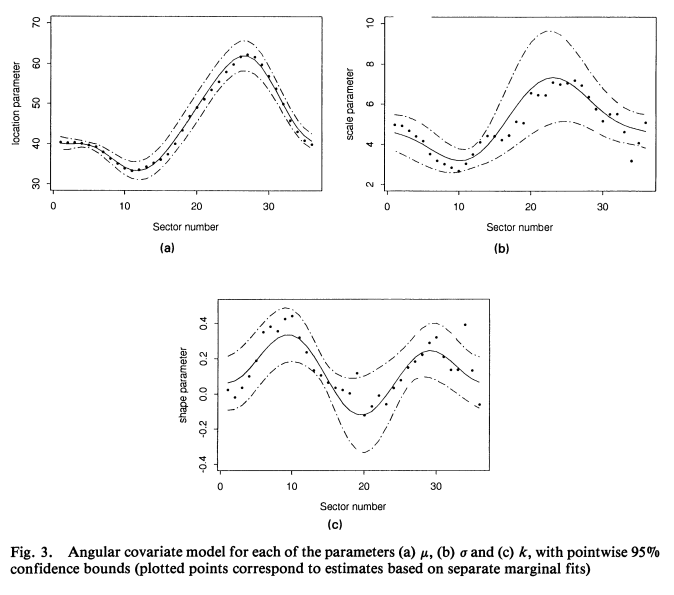
\includegraphics[scale=0.5]{estimation_param}
	
\end{frame}

\section{Modélisation de la dépendance angulaire}
\begin{frame}{Motivations}
	blabla
\end{frame}
\begin{frame}{GEV généralisé de Haan}
	
\end{frame}
\begin{frame}{Paramètres}

\end{frame}
\section{Estimation des paramètres de la dépendance angulaire}
\begin{frame}{$\theta$}

\end{frame}
\begin{frame}{$\xi$}

\end{frame}
\begin{frame}{graphique}

\end{frame}
\begin{frame}{Conclusion}
	
\end{frame}


	

			

%				\begin{frame}{References}
%					%\nocite{*}
%					%	\printbibliography
%					\bibliographystyle{amsalpha}
%					\bibliography{bibli1}
%				\end{frame}

				
\end{document}